\documentclass[a4paper]{article}
\usepackage[utf8]{inputenc}
\usepackage[french]{babel}
\usepackage[T1]{fontenc}
\usepackage{amsmath}
\usepackage{amssymb}
\usepackage{amsthm}
\usepackage{listings}
\usepackage{enumitem}
\usepackage{relsize}
\usepackage{dsfont}
\usepackage{graphicx}
\usepackage[margin=1in]{geometry}

\newcommand{\K}{\ensuremath\mathbb{K}}
\newcommand{\N}{\ensuremath\mathbb{N}}
\newcommand{\Z}{\ensuremath\mathbb{Z}}
\newcommand{\Q}{\ensureFmath\mathbb{Q}}
\newcommand{\R}{\ensuremath\mathbb{R}}
\newcommand{\U}{\ensuremath\mathbb{U}}
\newcommand{\C}{\ensuremath\mathbb{C}}
\newcommand{\E}{\ensuremath\mathbb{E}}
\newcommand{\V}{\ensuremath\mathbb{V}}
\renewcommand{\P}{\ensuremath\mathbb{P}}

\renewcommand{\(}{\left(}
\renewcommand{\)}{\right)}

\newcommand{\la}{\leftarrow}
\newcommand{\xla}{\xleftarrow}
\newcommand{\ra}{\rightarrow}
\newcommand{\xra}{\xrightarrow}

\renewcommand\labelitemi{---}

%\setlength\parindent{0pt}

\newtheorem*{definition}{Définition}
\newtheorem*{theorem}{Théorème}
\newtheorem*{algo}{Algorithme}
\renewcommand*{\proofname}{Preuve}

\title{Rapport: ReactiveRS2}
\author{Thibaut Pérami, Mathieu Fehr}

\begin{document}

\maketitle

\section{Introduction}

Pour ce projet de programmation parallèle et réactive, nous avons d'abord écrit
une première version (qui n'a pas été finie), en suivant la structure proposée
dans les TP.

Cependant, nous avons ensuite décidé de changer la structure de la bibliothèque.
Nous pensons que cette nouvelle structure permet d'être plus efficace, et offre
une représentation des programmes réactifs plus intuitive. Cependant, cette
nouvelle structure est plus difficile à programmer (en Rust), plus
lente à compiler, et pose quelques
problèmes pour l'écriture des fonctions and\_then et flatten (que nous n'avons
pas codés par souci de temps).

\section{Fonctionnement de la bibliothèque}

La bibliothèque repose non pas sur un vecteur de continuations, mais sur un
graphe de flot de contrôle. 

\subsection{Noeuds}

Un noeud de ce graphe est essentiellement une opération élémentaire
réactive. L'exécution d'un noeud peut être l'exécution d'une fonction non
réactive (comme une FnMut ou une FnOnce), une pause, une émission d'un signal, un
await d'un signal, etc... Un noeud possède une entrée et une sortie, afin de
passer des valeurs dans le programme. L'exécution d'un noeud est toujours
instantanée, par exemple le noeud \verb!NPause! se contant de mettre le numéro
du noeud suivant dans la liste des noeuds à exécuter à l'instant suivant.

Pour stocker des noeuds dans le graphe, il faut qu'ils aient le même type. Pour
cela, nous ne stockons que des noeuds prenant en entrée () et en sortie ().
Cela nous oblige à passer par des Rc<Cell> ou des Arc<Mutex> pour passer des
valeurs, ce qui ralentit l'exécution du code. Pour remédier à ce problème, nous
pouvons associer deux noeuds séquentiellement dans un même noeud, pour pouvoir
par exemple appliquer la fonction f(g(x)) dans un même noeud, au lieu de passer
g(x) dans un Rc/Arc, pour le passer au noeud contenant f.

Pour savoir quels noeuds sont exécutés, nous stockons simplement dans un tableau
la liste des noeuds à exécuter à l'instant courant, et à l'instant suivant.

Pour simplifier l'écriture de ce graphe et garantir statiquement certain
invariant dessus (par exemple qu'une FnOnce n'est appelé qu'une seule fois),
l'utilisateur n'a pas à utiliser les noeuds directement, et utilise une autre
structure: les processus.

\subsection{Processus}
Un processus permet à l'utilisateur de manipuler des opération réactive
non-instantanée en un seul bloc. Cela permet de ne pas toujours réécrire les mêmes
blocs, et d'avoir une compilation efficace vers le graphe de noeuds.

Un processus possède aussi une entrée, et une sortie et contrairement à un
noeud, représente un calcul qui peut s'étaler sur plusieurs instants.
Il y a deux types de
processus: les processus immédiats et les processus non immédiats. Les processus
immédiats se compilent en un unique noeud, tandis que les processus non
immédiats se compilent en plusieurs noeuds, dont un d'entrée et de sortie.
L'utilité de cette structure est que plusieurs processus immédiats compilés
séquentiellement peuvent se composer statiquement en un unique noeud, contenant la séquence
de tout les noeuds immédiats, et réduisant ainsi le nombre de Rc/Arc utilisés.
Ainsi, si un processus non immédiat est compilé en 3 noeuds (Nentrée, Nmilieu,
Nsortie), et est mis en séquence avec un noeud immédiat (Nimmédiat), alors
il aura son noeud Nsortie fusioné avec Nimmédiat.
Cela permet d'avoir un minimum de Rc/Arc utilisés. Pour plus d'exemple, cf la
partie sur les exemples de structures.

\subsection{Signaux}

Les signaux utilisent l'attente passive pour pouvoir effectuer les actions. Cela
permet de ne pas avoir à effectuer des calculs pour un signal lorsque celui-ci
n'est pas utilisé. Pour cela, on garde en mémoire les deux derniers instants
dans lesquels un signal à été émis, et on ne met a jour le signal que lorsqu'on
interagit avec lui (à travers un emit, ou lorsqu'on récupère sa valeur).

\subsection{Macros}

Pour simplifier l'écriture d'un programme réactif, nous avons utilisé des macros
procédurales. Ces macros, écrites dans une crate à part, permettent d'avoir une
syntaxe plus simple, en réduisant l'imbrication. La macro parcours un arbre
post-lexage (les seule chose qui y sont parsés sont le paires de délimiteurs),
et en déduit comment générer un code Rust adapté à la bibliothèque.

\subsection{Parallélisation}

Pour paralléliser, on a découpé le \verb!Runtime! en $n$ \verb!ThreadRuntime!,
chacun tournant sur un worker-thread. La synchronisation entre les worker-thread
se fait de manière totalement lock-free:

Chaque worker-thread a 3 files de work-stealing (chase-lev) qui correspond aux
instants congrus a 0,1 et 2 modulo 3. Il a de la même façon 3 nombres atomiques \verb!nbf! qui
représentent le nombre de threads qui ont fini l'instant.

Dans un instant, on garde la notion d'ownership d'un noeud qui est passé à
travers les file de work-stealing. De par la structure de graphe générée par les
processus, on a la garantie qu'un numéro de noeud ne peut jamais être plusieurs
fois dans dans les file d'attente. On a donc bien la notion d'ownership.

\paragraph{Synchronisation :} On maintient donc l'invariant suivant: à tout
moment notre thread n'est pas compté comme
fini dans \verb!nbf! si il possède au moins un noeud devant être exécuter à cet
instant. Pour conserver cet invariant, Un thread, lorsqu'il fini sa
file de noeud va incrémenter de 1 \verb!nbf! mais il le baissera de 1 avant
toute tentative de vol (on essaie de voler que dans les files non-vide). De cette
manière lorsque \verb!nbf! atteint $n$, on sait que plus aucun thread ne possède
de noeud associé à l'instant courant on peut changer d'instant.

Lorsqu'on change d'instant, certain threads qui ont \og vu\fg{} la valeur de $n$
dans le \verb!nbf! de l'instant $i$, vont commencer à exécuter les noeud de l'instant $i+1$ et
peuvent potentiellement ajouter des noeuds au files des instant $i+1$ et $i+2$ .
Or les threads qui n'ont pas encore remarqué que l'on avait changé d'instant
vont continuer a tenter de voler dans le file de l'instant $i$. If faut donc que
les files de l'instant $i$, $i+1$, $i+2$ soient différentes.

De même un thread qui est dans l'instant $i+1$ peut atteindre le moment où il
doit incrémenter le \verb!nbf! de l'instant $i+1$ avant que tout les thread se
soit rendu compte qu'on ait commencé l'instant $i+1$, et vont bien se baser sur
le fait que le \verb!nbf! de l'instant $i$ vale $n$ pour changer d'instant. Il
faut donc au moins 2 \verb!nbf! différent. Il reste donc le problème de
réinitialiser \verb!nbf! à un moment où cela ne pose pas de problème. Je garde
donc 3 \verb!nbf! différent et le \verb!nbf! de l'instant $i-1$ i.e de l'instant
$i+2$ est réinitialisé par tout thread passant de l'instant $i$ à l'instant $i+1$.

On peut ainsi passer d'un instant à l'autre de manière synchronisé mais lock-free

\paragraph{Deadlock:} Voyons maintenant pourquoi un deadlock ne peut pas se produire


\subsection{Optimisation à coup d'invariant satiques}

\section{Améliorations possibles}

Par manque de temps, du à des complications avec Rust, nous n'avons pas pu
écrire certaines structure. Nous présentons ici des idées d'implémentation pour
ces structures:

\begin{itemize}
\item Flatten: Puisque la bibliothèque se base sur une compilation du programme
  réactif, il est difficile d'implémenter des processus produits dynamiquement.
  Cependant, nous avons une idée d'implémentation. L'idée serait d'avoir un
  noeud prenant en entrée un processus, et compilant ce processus, pour contenir
  un sous-graphe. Le noeud contiendrait aussi un runtime, pour savoir quels
  noeuds sont à exécuter.
\item Structures de controle récatif comme \verb!do until!. On les avait
  initialement fait sur une version ancienne, mais après de multiple refactorings
  du système de processus pour atteindre des temps de compilation raisonnables,
  nous n'avons pas eu le temps et la motivation de leur faire suivre tout les changements.
\end{itemize}

\section{Exemple de compilation de structure de contrôle}

\subsection{Branche parallèle :}

Voici un exemple de petit processus parallèle:
\begin{verbatim}
|_| (0,0);
{
    {
        |_| 20;
        Pause;
        |i| i+1;
        Pause
    } || {
        |_| 20;
        Pause;
        |i| i+1;
        Pause
    }
};
|(v1,v2)| v1 + v2;
Pause;
|i| {
    ()
}
\end{verbatim}

et en voici la compilation en noeud (Rust mettant 12 minutes à compiler cet
exemple avec 12Go de RAM, Je n'ai pas eu le temps de générer la version processus):
\begin{center}
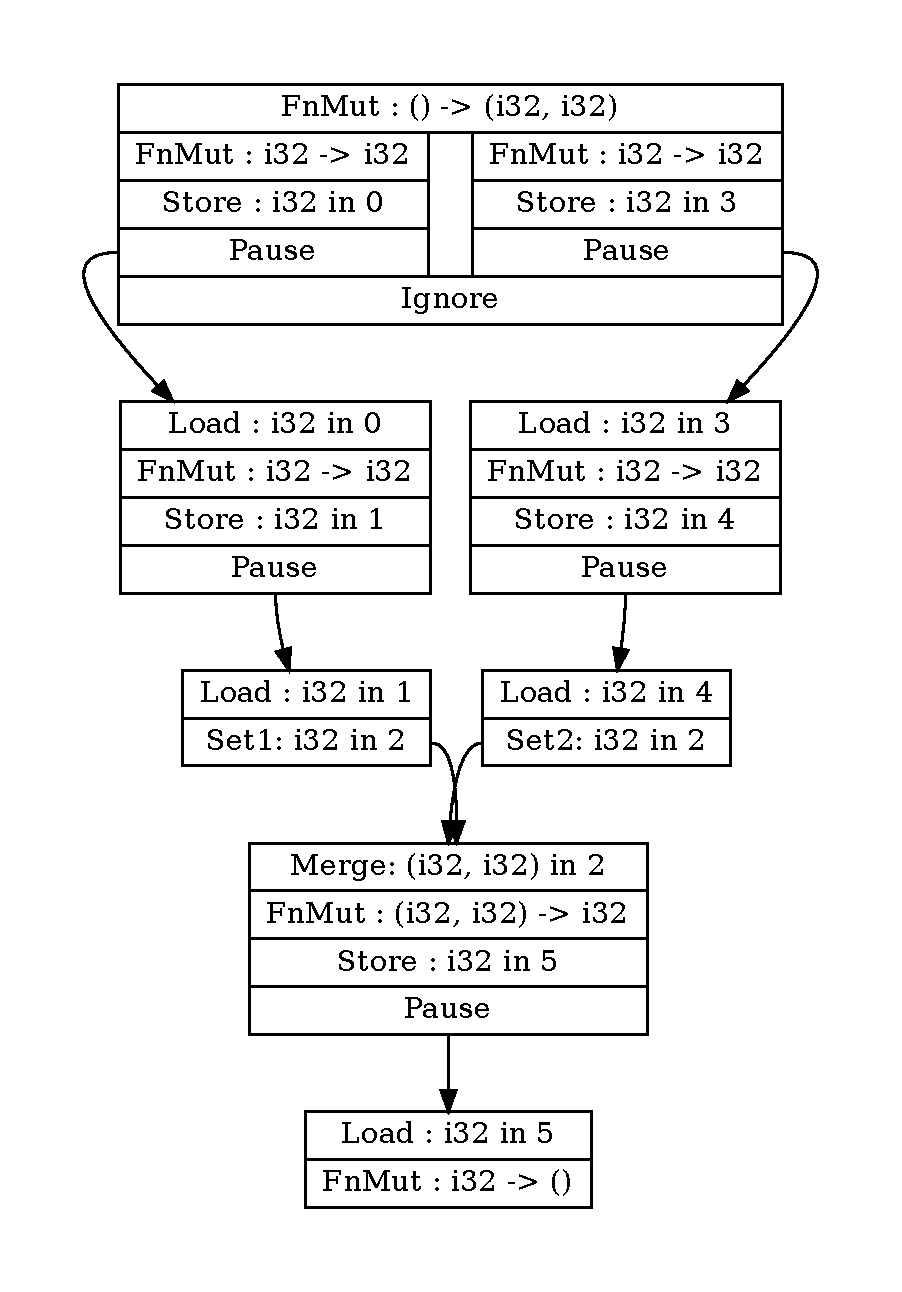
\includegraphics[scale=0.8]{test.pdf}
\end{center}


\subsection{Boucle :}

\begin{verbatim}
|_| 0;
loop {
    |i|{
        if i < 42{
            True(i+1)
        }
        else {
            False(i)
        }
    };
    Pause
};
|i| ()
\end{verbatim}

En processus, on a :
\begin{center}
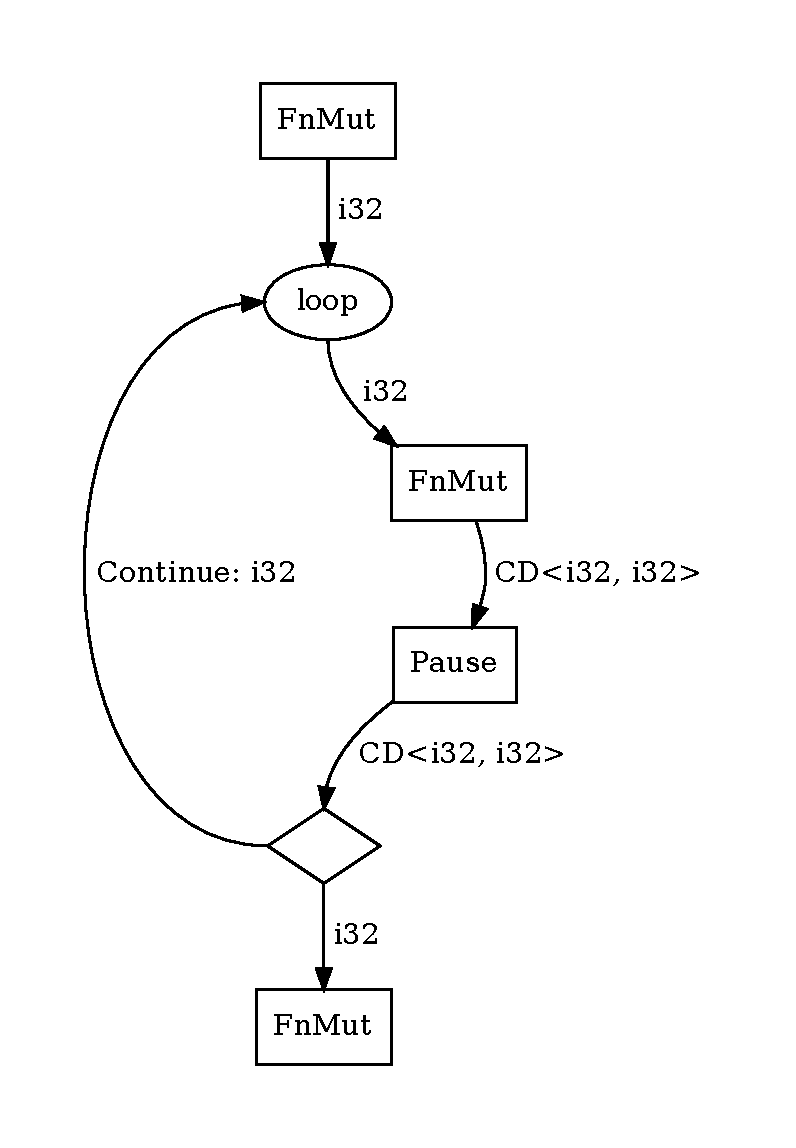
\includegraphics[scale=0.72]{loopp.pdf}
\end{center}

Et un fois compilé vers les noeuds, on a:
\begin{center}
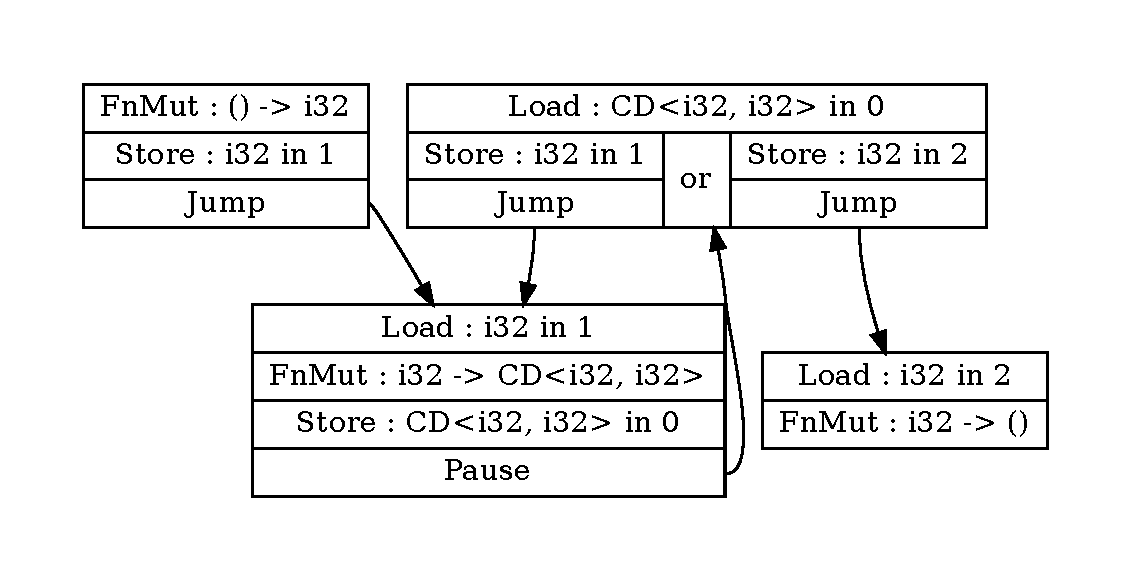
\includegraphics[scale=0.72]{loopn.pdf}
\end{center}


\section{Exemple d'application}

En idée d'application simple hautement parallèle, nous avons pensé au jeu de la
vie. Pour utiliser au maximum l'aspect réactif, nous avons utilisé des signaux
pour faire communiquer les cases entre elles. Chaque case contient un signal, et
lorsque la case est allumée, elle envoie un signal a toute ses cases voisines.
La réception des signaux permet alors de calculer l'étape suivante. La
structure, étant sparse, n'a pas besoin de calculer la valeur d'une case lorsque
celle ci ne possède pas de voisins allumés. Pour afficher un état, nous
utilisons un signal qui est émis pour chaque case allumée. Ce signal contient
donc l'état du tableau.

\section{Liste (non exhaustive) de problèmes avec Rust}
\subsection{Bug}
Nous avons rencontré plusieurs fois des crash du compilateur sans message d'erreur
autre que \og unexpected panic\fg{}. Cela ralentit beaucoup le temps de
développement de dichotomiser sur des ligne de code en les commentant ou pas
pour trouver laquelle fait planter le compilateur.


\subsection{Trait A ou B}
-Il est impossible de spécifier une somme d'interface au compile time. En effet
on dispose, pour les types, de type produits \verb!(A,B)! et de type sommes
\verb!enum{A(A), B(B)}!. Mais on ne pas faire cela avec des interfaces. Pour les
produit d'interface, cela ne pose pas de problème, il suffit de créer un
interface demandant \verb!A! et \verb!B! : \verb!trait C : A + B!.
Malheureusement il n'est pas possible de définir d'interface somme: Un type
rentre dans l'interface $C$ si il vérifie celle de $A$ ou celle de $B$ et qu'on
peut lui associer celle des 2 qu'il vérifie (en cas de doublon). Nous avons donc du
bidouiller le système de type avec des type de marquage et des méthodes
inactives (qui paniquent quand on les appelle), mais il serait agréable
que cela soit intégré au langage.

\subsection{Inférence de type}
-L'algorithme de compilation semple mettre un temps exponentiel en la profondeur
des types paramétriques: le système de type générique de Rust semble donc inutilisable
pour des exemple non triviaux (autre que Vec et Box en gros).

\section{Conclusion}
La difficulté de faire comprendre certain concepts au système de type de Rust et
l'explosion des temps de compilation qui en a suivi nous a empêché de terminer la
parallélisation de notre bibliothèque à temps. Nous avons probablement trop
voulu faire d'optimisation au compile-time sans vérifier si rustc avait la
capacité de les supporter efficacement.


\end{document}